
\section{Integrating Multiphysics}

Consider a system whose evolution depends on several different
physical processes, represented by the operators $A$, $D$,
$R$ (advection, diffusion, and reactions, respectively).
\begin{equation}
\phi_t = -A(\phi) + D(\phi) + R(\phi)
\end{equation}
One way to solve this system is to discretize each of the operators in
space.  For instance the discrete advection operator, $[A(\phi)]_i$
might use the ideas on piecewise linear reconstruction techniques
discussed in chapter~\ref{ch:advection}, $[D(\phi)]_i$ can use the
discrete form of the Laplacian from chapter~\ref{ch:diffusion}, and
$[R(\phi)]_i$ may be an algebraic relation.  This leaves us with an ordinary differential equation for the time-evolution of $\phi$,
\begin{equation}
\frac{d\phi_i}{dt} = -[A(\phi)]_i + [D(\phi)]_i + [R(\phi)]_i
\end{equation}
which can be solve using standard ODE techniques.  This is the {\em
  method of lines} technique we saw with advection
(\S~\ref{adv:sec:mol_2d}) and compressible hydrodynamics
(\S~\ref{sec:comp:mol}), and can be a powerful technique to solve PDEs
or systems of PDEs with multiple physics operators

A difficulty arises if these processes each have different timescales
associated with them.  For instance, reactions may be vigorous and
require a small timestep to accurately capture the changes, but the
advection is slow.  Or, recall that the timestep limiter for explicit
diffusion scales as $\Delta x^2$ while explicit advection scales as
$\Delta x$, so these processes could demand very different timescale
for evolution.  Therefore, we don't want to use the same timestep for
all the processes, since that will needlessly make things
computationally expensive.  {\em Operator splitting} solves for the
effects of each operator separately, using whichever timestep (and
time-discretization, e.g., explicit or implicit) is most suited to the
operation.  The result of one operation is used as the input to the
next\footnote{This directly parallels the dimensional splitting
  approach we saw for advection in \S~\ref{adv:sec:dimensionalsplit}}.
The downside of this approach is that the operations may not be well
coupled.


\section{Ex: diffusion-reaction}
\label{sec:multiphys:diffreact}

Consider a diffusion-reaction equation:
\begin{equation}
\phi_t = \kappa \phi_{xx} + \frac{1}{\tau} R(\phi)
\end{equation}
This can be thought of as a simple model for a combustion flame, and
can propagate a front.  It is often the case that the reactions are
stiff, and require a smaller timestep then the diffusion part.  In
fact, we may want to use an implicit integration method designed for
stiff ODEs for the reaction part, but use a standard explicit method
for the diffusion part.  This requires operator splitting.

We can use Strang splitting \cite{strang} to make the integration
second-order accurate overall:
\begin{equation}
\phi^{n+1} = R_{\Delta t/2} D_{\Delta t} R_{\Delta t/2} \phi^n
\end{equation}
where $R_{\Delta t/2}$ represents reacting for a step of $\Delta t/2$
and $D_{\Delta t}$ represents diffusing for a step of $\Delta t$.  In
each case, these operators act as if the other were not present, but
they see the effect of the previous operation on the input $\phi$.  
Note that no explicit source terms describing one process appear in the other
process's update.  The procedure for updating appears as:
\begin{enumerate}
\item {\em Evolve reaction ODE system for $\Delta t/2$}

  Define $\phi^\star$ as the the solution to the ODE:
   \begin{equation}
     \frac{d\phi}{dt} = \frac{1}{\tau} R(\phi), \quad 
   \phi(t^n) = \phi^n, \quad t \in [t^n, t^{n+\myhalf}]
   \end{equation}

\item {\em Solve the diffusion equation for $\Delta t$ with an
           implicit Crank-Nicolson discretization}
   %
   \begin{equation}
     \frac{\phi^{\star\star} - \phi^\star}{\Delta t} =
      \frac{1}{2} (D(\phi^\star) + D(\phi^{\star\star}))
   \end{equation}

   Note that the starting point is $\phi^\star$.

\item {\em Evolve reaction ODE system for $\Delta t/2$}

  Define $\phi^{n+1}$ as the the solution to the ODE:
   \begin{equation}
     \text{define } \phi^{n+1}: \, \frac{d\phi}{dt} = \frac{1}{\tau} R(\phi), \quad 
   \phi(t^{n+\myhalf}) = \phi^{\star\star}, \quad t \in [t^{n+\myhalf}, t^{n+1}]
   \end{equation}

\end{enumerate}

Consider a simple reaction source
\begin{equation}
  \label{eq:multiphysics:react}
  R(\phi) = \frac{1}{4} \phi (1 - \phi)
\end{equation}
This is called a KPP reaction source.  Here $\phi$ can be thought of
as a progress variable that varies between pure ash ($\phi = 0$) and
pure fuel ($\phi = 1$).  Figure~\ref{fig:diffreact} shows the solution
to our diffusion-reaction equation with 256 zones, $\kappa = 0.1$,
$\tau = 1.0$ at several times.

\begin{figure}[t]
\centering
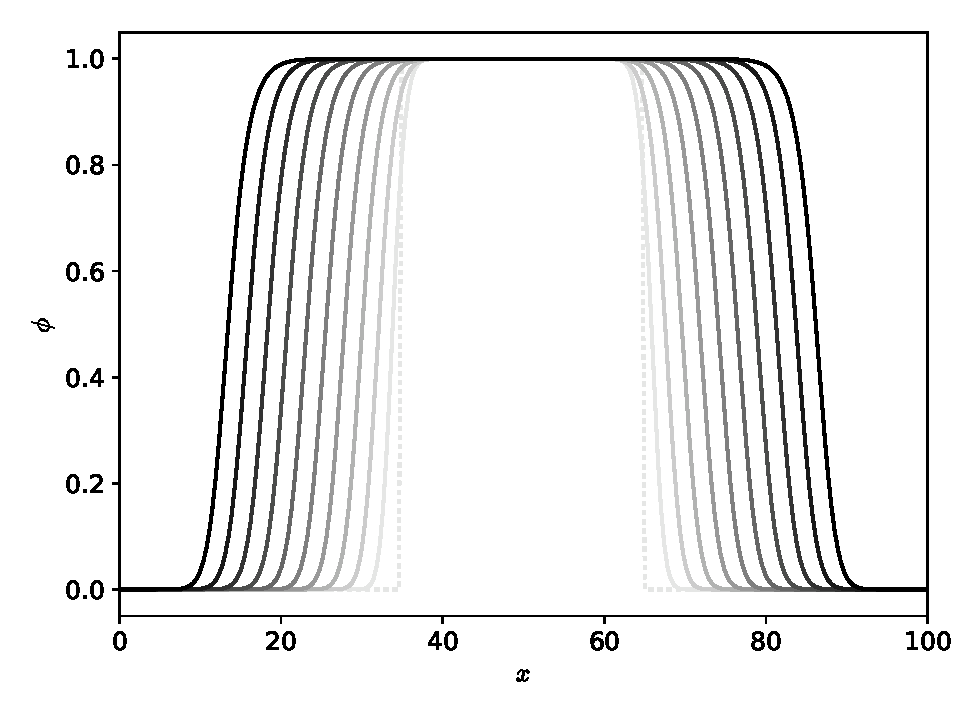
\includegraphics[width=5.0in]{flame_seq}
\caption[Solution to the diffusion-reaction equation]
  {\label{fig:diffreact} Solution to the diffusion-reaction equation
   with 256 zones, and $\kappa = 0.1$, $\tau = 1.0$.  The lines shown
   are spaced 8.0 time-units apart.  We see the initial smoothed tophat
   profile giving rise to a traveling front. \\
   \hydroexdoit{\href{https://github.com/zingale/hydro_examples/blob/master/multiphysics/diffusion-reaction.py}{diffusion-reaction.py}}
   }
\end{figure}

 The solution in this case is a wave with speed $S = \sqrt{\kappa/\tau}$
 and thickness $\delta = \sqrt{\kappa \tau}$ (see \cite{vladimirova2006} for
 some details of this system).

\begin{exercise}[Diffusion-reaction system]
 Solve the the difusion reaction equation with the source given in 
 Eq.~\ref{eq:multiphyiscs:react}.  Note that you should begin with
 some smooth initial conditions---if they are too sharp than the 
 C-N discretization will cause jagged features to appear.  
 Compare your results to Figure~\ref{fig:diffreact}.
\end{exercise}


\section{Ex: advection-diffusion}

\label{ch:multiphysics:sec:adburgers}

The viscous Burgers' equation appears as:
\begin{equation}
u_t + u u_x = \epsilon u_{xx}
\end{equation}
This admits shocks and rarefactions just like the inviscid form we
studied in Chapter~\ref{ch:burgers}, but now the viscosity can act to
smooth out the shock---instead of being infinitely thin, it will have
a physical width.

As we saw earlier, there are efficient, accurate methods for handling
the advective parts explicitly, but for diffusion, we often want to 
solve it implicitly.  We can split the solution up, but couple the 
two processes together to make a method that is overall second-order
accurate in time.  We write our equation as:
\begin{equation}
u_t + A(u) = D(u)
\end{equation}
with $A(u) = [\frac{1}{2} u^2]_x$ and $D(u) = \epsilon u_{xx}$.  Then our update 
appears in two steps.
\begin{enumerate}
\item {\em Find the advective update over the timestep}:
   We use an approximation of the diffusion term at time-level $n$, $D(u^n)$
   as a source in the construction of the interface states for the 
   advective part.  Once the interface states, $u_{i+\myhalf}^{n+\myhalf}$ are
   known, we construct the advective update term as:
   \begin{equation}
   A_i^{n+\myhalf} = 
     \frac{\left [ \frac{1}{2} \left (u_{i+\myhalf}^{n+\myhalf}\right)^2\right ] -
           \left [ \frac{1}{2} \left (u_{i-\myhalf}^{n+\myhalf}\right)^2\right ]}
          {\Delta x}
    \end{equation}

\item {\em Solve the diffusion equation with the advective source}:
    We use a Crank-Nicolson discretization of the diffusion part of 
    our equation, with the advective update term appearing as a source.
    \begin{equation}
    \frac{u^{n+1} - u^n}{\Delta t} = 
        \frac{1}{2}D(u^n) + \frac{1}{2}D(u^{n+1}) - A^{n+\myhalf}
    \end{equation}
    
    This is a linear system that can be solved as a tridiagonal matrix
    or with multigrid.  The result of this step is that $u^{n+1}$ is
    updated with both the advection and diffusion terms.

\end{enumerate}

Because the diffusion is done implicitly, the timestep constraint (for
stability) for this solve is due to the advective portion only.

\begin{figure}[t]
\centering
\includegraphics[width=5in]{burgersvisc}
\caption[Viscous Burgers' equation solution]
  {\label{fig:viscburger} Solution to the viscous Burgers' equation
  with a variety of different viscosities.  The initial conditions was
  a single wavelength of a sine wave for $x \in [1/3,2/3]$, and $u = 1$
  otherwise. \\
  \hydroexdoit{\href{https://github.com/zingale/hydro_examples/blob/master/multiphysics/burgersvisc.py}{burgersvisc.py}}}
\end{figure}

For step 1, the addition of the explicit diffusion source requires
a small change to the method we used to predict the interface states.

\begin{eqnarray}
u^{n+1}_{i+\myhalf,L} &=& u^n_i + \frac{\Delta x}{2} \frac{\partial u}{\partial x}
                        + \frac{\Delta t}{2} \frac{\partial u}{\partial t} + \ldots \\
                &=& u^n_i + \frac{\Delta x}{2} \frac{\partial u}{\partial x}
                        + \frac{\Delta t}{2} \left (-u_i \frac{\partial u}{\partial x} + D(u^n_i) \right ) + \ldots \\
                &=& u^n_i + \frac{\Delta x}{2} \left ( 1 - \frac{\Delta t}{\Delta x}u_i \right ) \frac{\partial u}{\partial x} + {\color{red} \frac{\Delta t}{2} D(u^n) } + \ldots
\end{eqnarray}
here the source term (shown in red) incorporates the effects of the
diffusion on the prediction of the states for advection.  This entered
into our states when we replaced $\partial u/\partial t$ with our PDE
equation.  The spatial derivative, $\partial u/\partial x$ is replaced
by a monotonized difference, and the method then proceeds as with the
regular Burgers' equation.  The Riemann problem is unchanged from the
inviscid case.

Figure~\ref{fig:viscburger} shows the solution of the viscous Burgers'
equation for shock initial conditions with different amounts of
viscosity.  Notice that the effect of the viscosity is to smooth the
shock profile, but the shock position itself agrees between the cases.


\subsection{Convergence without an analytic solution}

Assessing the convergence of this is more difficult than the tests we
looked at before, since there is no analytic solution to compare to.
In this case, we can compare a very high-resolution solution and take
this to be the {\em right} answer / benchmark solution, and then
compare coarser simulations to a coarsened version of the benchmark solution.
This is done in Figure~\ref{fig:multiphysics:burgersconverge}.  The
fine zones of the benchmark are averaged into a corresponding coarse grid zone
to produce a coarsened representation of the benchmark, and the norm 
of the error with the coarse simulation is computed.

\begin{figure}[t]
\centering
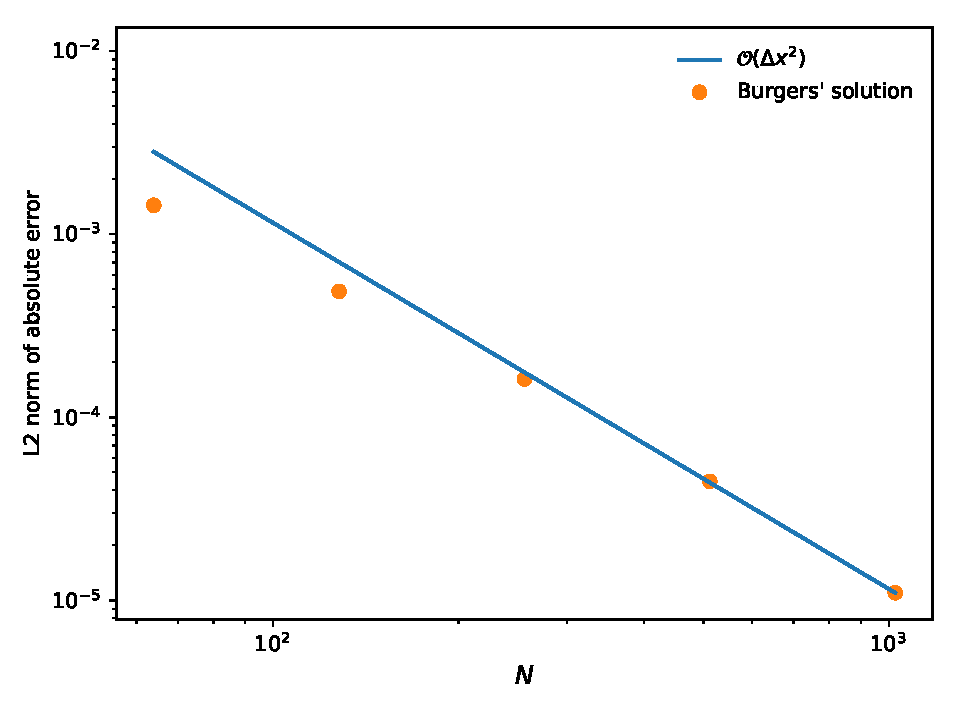
\includegraphics[width=5.0in]{burgersvisc_converge}
\caption[Convergence of the viscous Burgers' equation]
  {\label{fig:multiphysics:burgersconverge} Convergence of the Burgers'
    solution with $\epsilon = 0.005$.  To test convergence a run with 4096
    zones was done as a benchmark solution.  We see second-order
    convergence for the higher-resolution runs in this sample.\\
   \hydroexdoit{\href{https://github.com/zingale/hydro_examples/blob/master/multiphysics/burgersvisc_converge.py}{burgersvisc\_converge.py}}
   }
\end{figure}
